\chapter{Analisi dei Tempi}
In questa sezione della relazione si riporteranno i grafici delle misurazioni dei tempi.
\\I grafici mettono sempre in relazione i due algoritmi, distinguibili con il colore rosso per il PeriodNaive e con il colore blu per il PeriodSmart.


\section{Grafico 1}
Il primo grafico mostra il comportamento dei due algoritmi in funzione di $n$.\\
Nell'asse delle ascissa troviamo n mentre nell'ordinata il tempo espresso in nanosecondi
%Giustificare magari con una breve frase per scelte implementative particolare es abbiamo scelto di misurare la dev standrard con un campione di 50 iterazioni perchè i grafici ci venivano meglio
\\Osservando il grafico ci si accorge che i punti iniziali presentano una maggior densità e diventano sempre meno densi al crescere di $n$. Questo perchè i campioni sono distribuiti con una distribuzione esponenziale.
\begin{figure}[h!]
    \begin{center}
        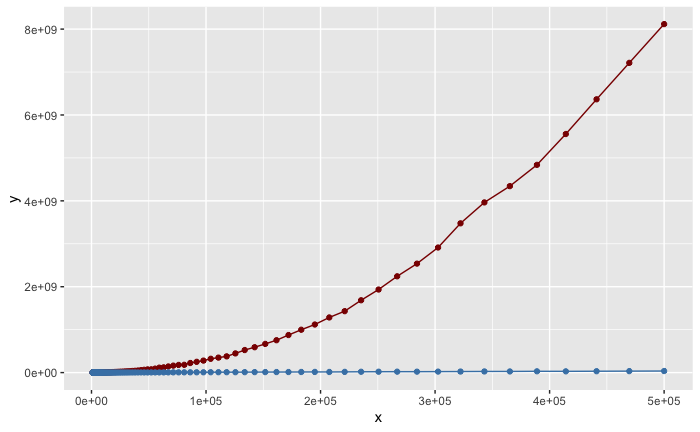
\includegraphics[width=170mm]{Grafico1}\\
    \end{center}
\end{figure}
\pagebreak


\section{Grafico 2}
Applichiamo al Grafico 1 una scala logaritmica per ogni asse. I campioni così risultano essere distribuiti in maniera ovviamente uniforme.
\\Da qui si nota la convenienza (traducibile in efficienza) del PeriodSmart rispetto al PeriodNaive, ad eccezione dei primi valori dove si evidenziano dei costi di overhead costanti.
\begin{figure}[h!]
    \begin{center}
        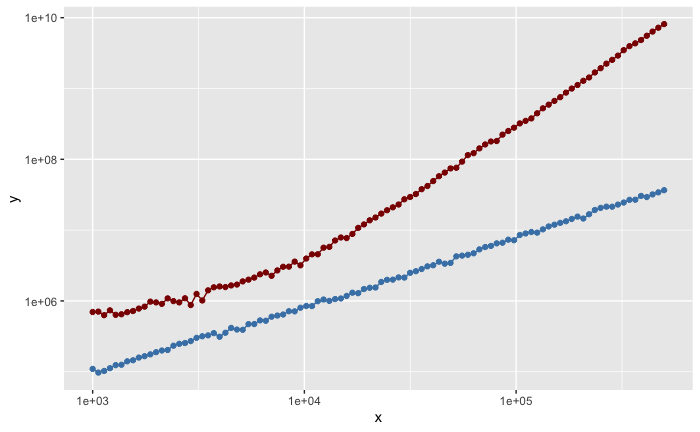
\includegraphics[width=170mm]{Grafico2}\\
    \end{center}
\end{figure}

%DISTRIBUZIONE PERIODO NON FATTA
%\section{Grafico 3 (Opzionale)}
%In questo grafico si evidenzia la distribuzione dei periodi calcolati per un n fissato. Stima dei periodi calcolati per le nostre stringhe
%opzionale e fatto con un altro programma che si può riportare in relazione con n = 100 es.
%Variante B (cambia il grafico se usiamo il metodo A o il B modificato con simbolo speciale)
%\begin{figure}[h!]
%    \begin{center}
%        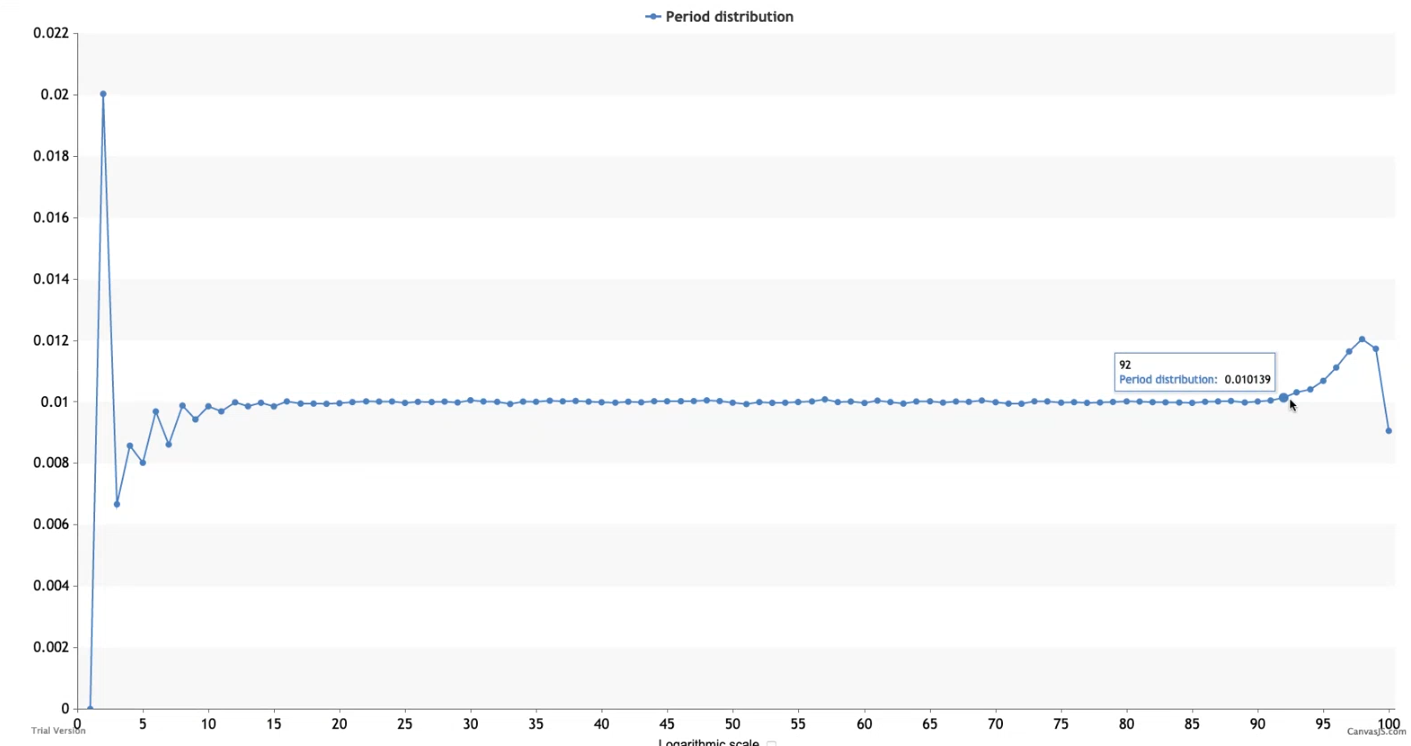
\includegraphics[width=130mm]{img/O1}\\
%    \end{center}
%\end{figure}


\pagebreak